\documentclass{article}

\usepackage{graphicx}
\usepackage{tikz}
\usepackage{tikzsymbols}
\usetikzlibrary{calc,patterns,shapes.geometric}
\pagestyle{empty}
\usepackage[margin=0pt]{geometry}
\geometry{papersize={14in,12in}}

\def\centerarc[#1](#2)(#3:#4:#5){\draw[#1] ($(#2)+({#5*cos(#3)},{#5*sin(#3)})$) arc (#3:#4:#5);}

\begin{document}
	\begin{figure}
		\centering
		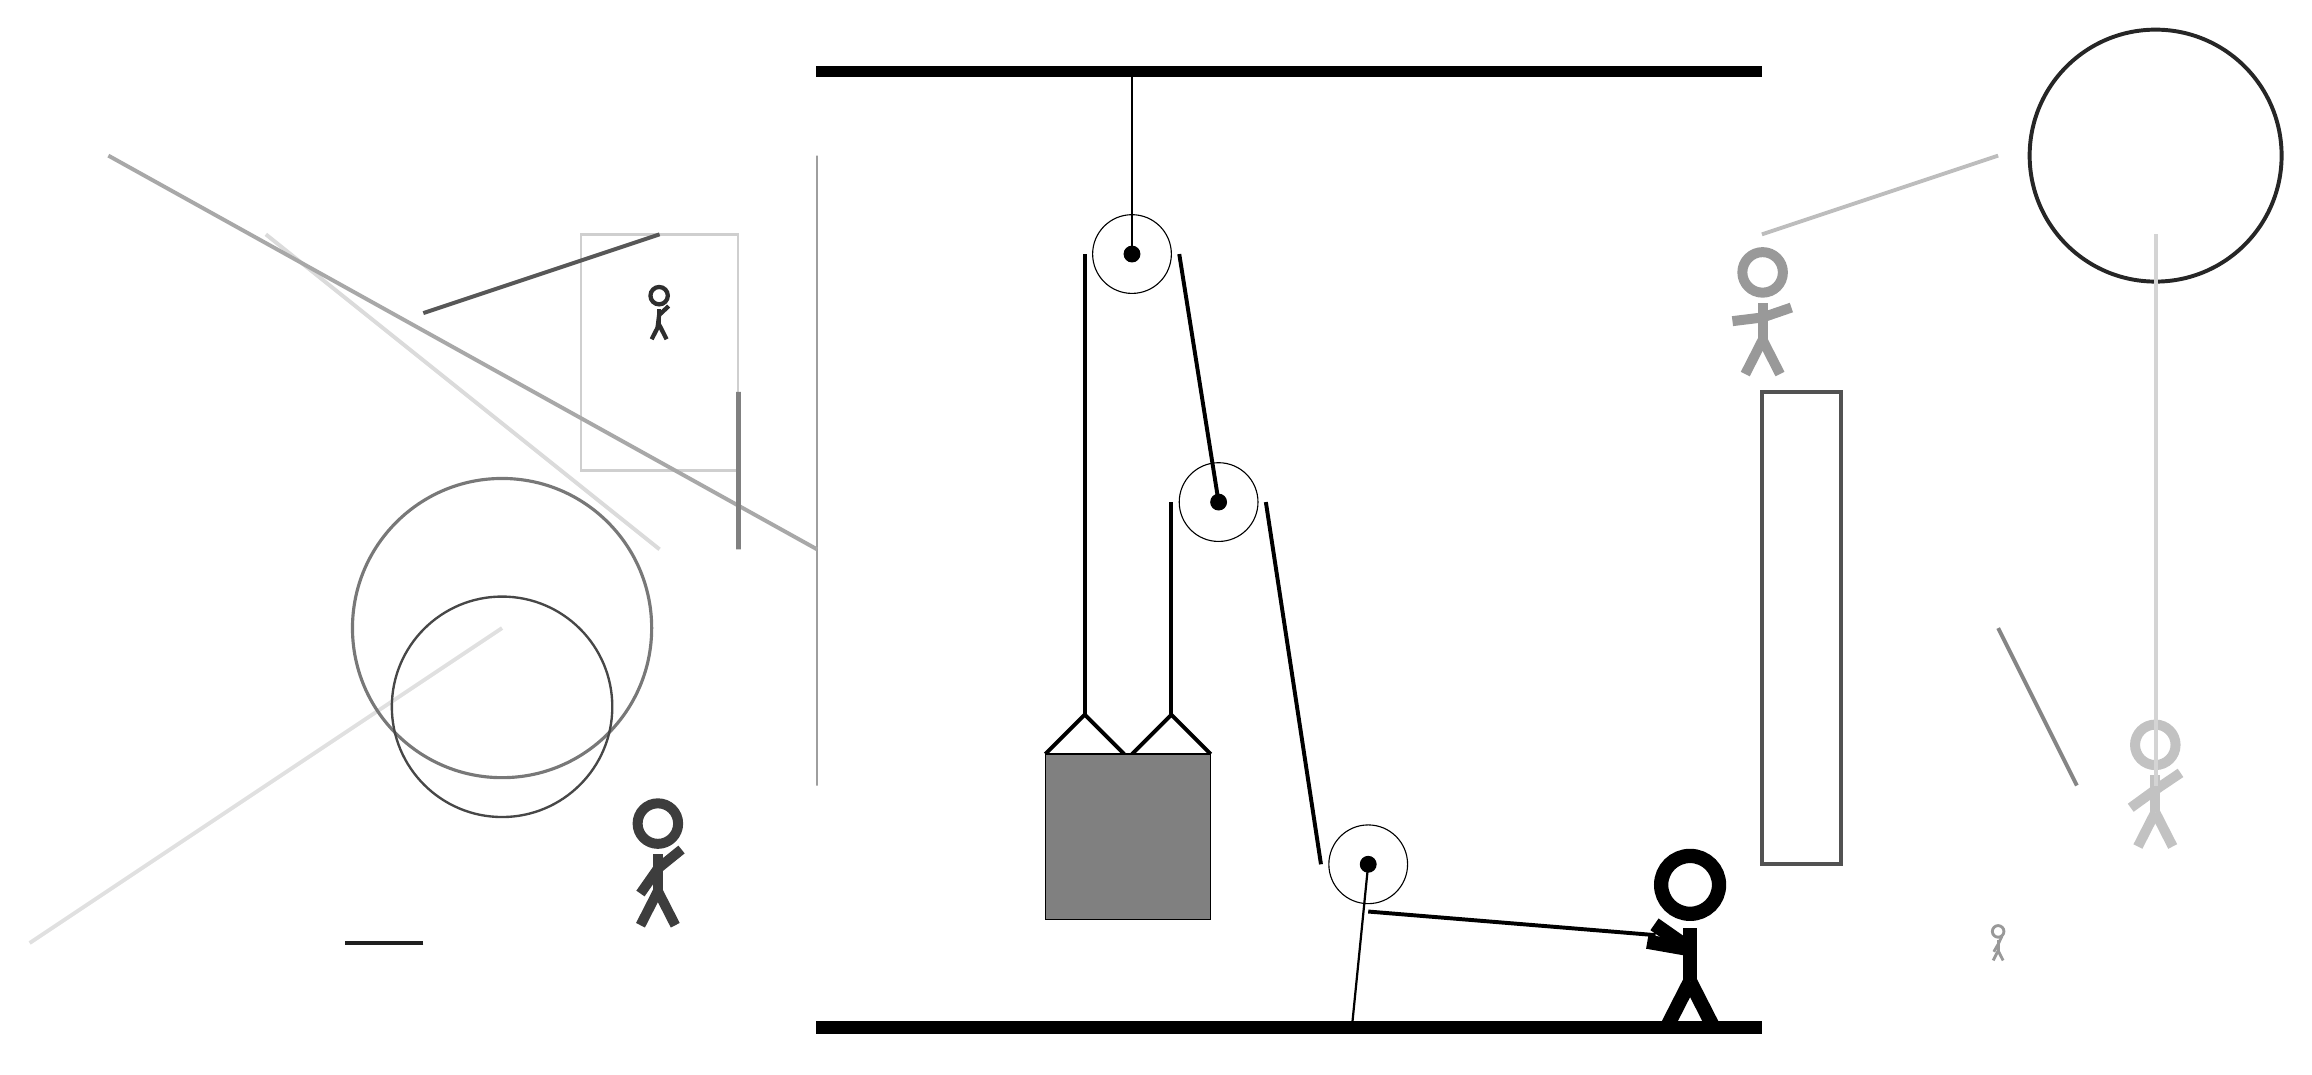
\begin{tikzpicture}
			%%%%% START %%%%%
			
			\draw[fill=black] (-2, 9) rectangle (10, 9.125);
			
			\draw (2, 6.75) circle (0.5);
			\draw[fill=black] (2, 6.75) circle (0.1);
			\draw[thick] (2, 6.75) -- (2, 9);
			
			\draw (3.1, 3.6) circle (0.5);
			\draw[fill=black] (3.1, 3.6) circle (0.1);
			
			\draw (5, -1) circle (0.5);
			\draw[fill=black] (5, -1) circle (0.1);
			\draw[thick] (5, -1) -- (4.8, -3);
			
			\draw[line width = 0.5mm]  (0.9, 0.4) -- (1.4, 0.9) -- (1.9, 0.4);
			\draw[line width = 0.5mm]  (2.0, 0.4) -- (2.5, 0.9) -- (3.0, 0.4);
			\draw[fill=black!50] (0.9, 0.4) rectangle (3.0, -1.7);
			
			\draw[line width = 0.5mm] (1.4, 6.75) -- (1.4, 0.9);
			\centerarc[line width = 0.5mm](2, 6.75)(0:180:0.6);
			\draw[line width = 0.5mm] (2.6, 6.75) -- (3.1, 3.6);
			\draw[line width = 0.5mm] (2.5, 3.6) -- (2.5, 0.9);
			\centerarc[line width = 0.5mm](3.1, 3.6)(0:180:0.6);
			\draw[line width = 0.5mm] (3.7, 3.6) -- (4.4, -1);
			\centerarc[line width = 0.5mm](5, -1)(180:270:0.6);
			\draw[line width = 0.5mm] (5, -1.6) -- (8.65, -1.9);
			
			\draw[line width=0.3mm, color=black!19] (-3, 7) rectangle (-5, 4);
			
			\draw[line width=0.5mm, color=black!68] (11, -1) rectangle (10, 5);
			\draw[line width=0.3mm, color=black!38] (-2, 0) rectangle (-2, 8);
			\draw [line width=0.4mm, color=black!26](15, 3) circle (0.0);
			\draw[line width=0.5mm, color=black!12](-6, 2) -- (-12, -2);
			\draw[line width=0.5mm, color=black!14](-4, 3) -- (-9, 7);
			
			\node[line width=0.4mm, color=black!24] at (15, 0) {\Strichmaxerl[7][36][34]};
			\draw[line width=0.5mm, color=black!34](-2, 3) -- (-11, 8);
			\draw[line width=0.5mm, color=black!66](-7, 6) -- (-4, 7);
			\node[line width=0.3mm, color=black!40] at (13, -2) {\Strichmaxerl[2][60][65]};
			\node[line width=0.6mm, color=black!40] at (10, 6) {\Strichmaxerl[7][7][19]};
			\draw[line width=0.5mm, color=black!48](14, 0) -- (13, 2);
			\draw[line width=0.5mm, color=black!26](10, 7) -- (13, 8);
			\node[line width=0.3mm, color=black!76] at (-4, -1) {\Strichmaxerl[7][55][39]};
			\draw [line width=0.5mm, color=black!85](15, 8) circle (1.6);
			\node[line width=0.3mm, color=black!82] at (-4, 6) {\Strichmaxerl[3][83][43]};
			
			\draw[line width=0.5mm, color=black!88](-7, -2) -- (-8, -2);
			\draw[line width=0.5mm, color=black!17](15, 7) -- (15, 0);
			\draw[line width=0.7mm, color=black!50] (-3, 5) rectangle (-3, 3);
			\draw [line width=0.4mm, color=black!53](-6, 2) circle (1.9);
			\draw [line width=0.3mm, color=black!72](-6, 1) circle (1.4);
			
			\node at (9, -2) {\Strichmaxerl[10][-35][170]};
			
			\draw[fill=black] (-2, -3) rectangle (10, -3.15);
			
			%%%%% END %%%%%
		\end{tikzpicture}
	\end{figure}	
\end{document}